\chapter{METHODOLOGY}
\section{Software Development Approach}
Agile development is a software development approach that emphasizes incremental progress and rapid cycles. It involves releasing small increments of functionality that build upon previous versions. Thorough testing is conducted for each release to ensure software quality. Agile is often employed for time-critical applications. Although this project is not time-critical this model seems to be the most optimal and practical in our case.
\begin{figure}[hbt!]
    \center{
        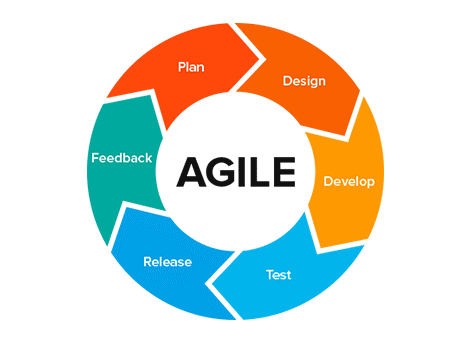
\includegraphics[width=0.75\textwidth]{./img/agile.png}
        \caption{Agile Model for Software Development}
        \subcaption*{\textit{source: \textcolor{blue}{https://mobilelive.medium.com/agile-development-a-comprehensive-guide-for-the-modern-era-d2fe9ae7b395}}}
    }
\end{figure}
\newpage
\section{Proposed System Block Diagram}
    \begin{figure}[hbt!]
    \center{
        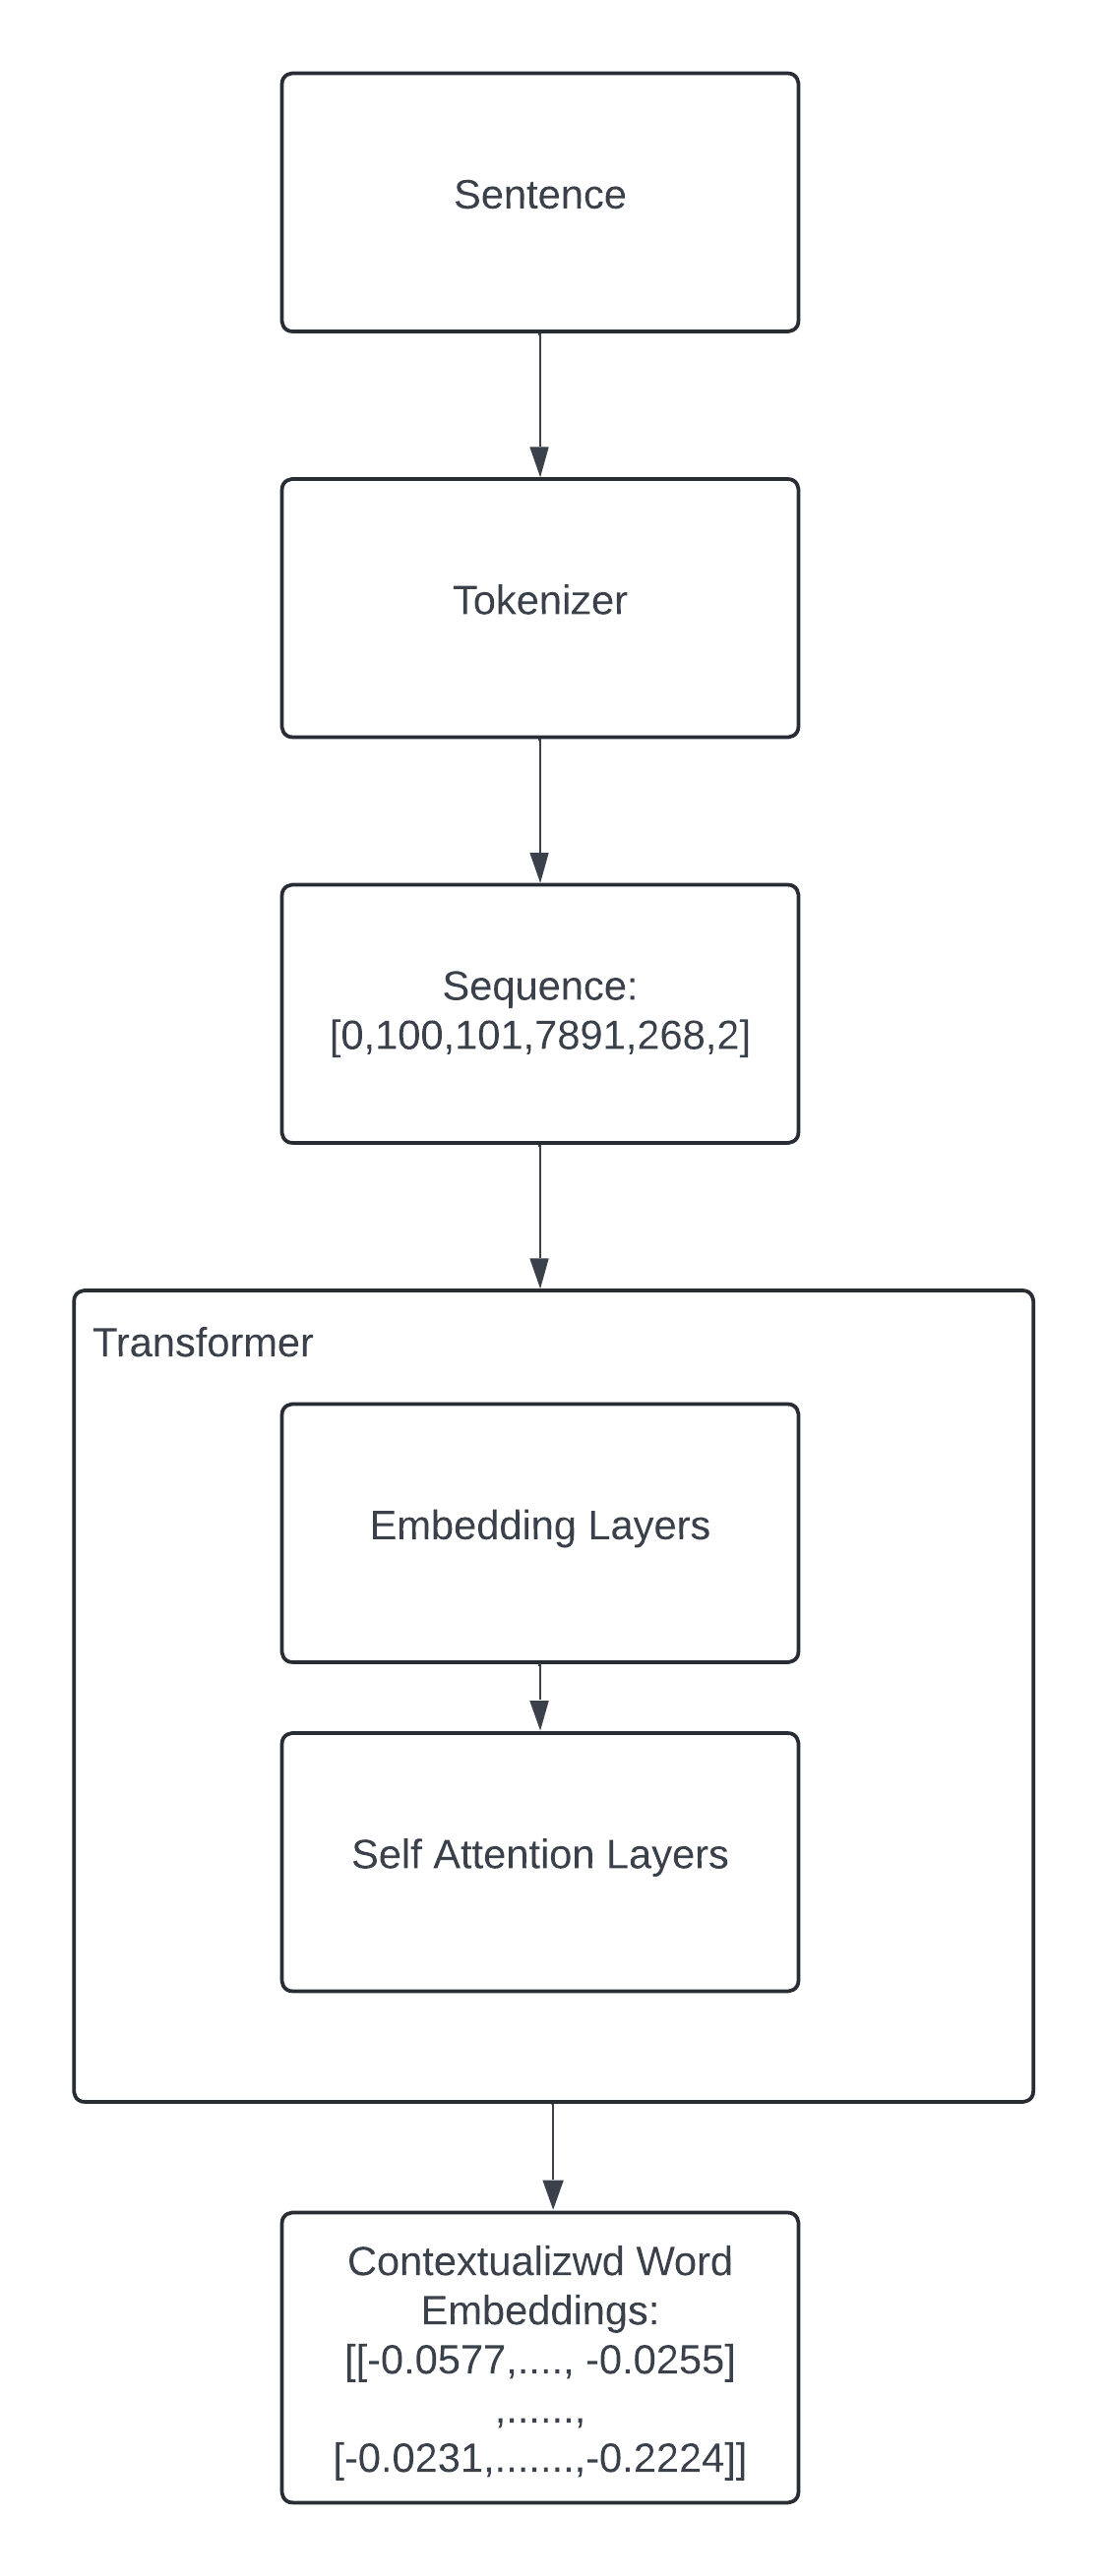
\includegraphics[width=0.6\textwidth]{./img/Block_Diagram.png}
        \caption{Block diagram of Proposed Sytem}
        }
    \end{figure}

\section{Description of Working Flow of Proposed System}
\section{Performance Evaluation Metrics}